% uid: ""
% school: "college"
% level: "7eme"
% chapter: "التناظر المحوري"
% chapter_slug: "symetrie-axiale"
% title: "مناظرات على الشبكة"
% difficulty: "Facile"
% tags: ["symetrie-axiale", "quadrillage", "construction", "longueurs"]
% provenance: "own"
% batch: "2026-11-27-symetrie-axiale-7eme"
% Exercice 2/10 de la série 7ème « التناظر المحوري » (statement + \axsol + solution). Compiler avec XeLaTeX + axiomath.sty (+ axiomaths-logo.png).
\documentclass[12pt,a4paper]{article}
\usepackage[level=7b,color=0F766E]{axiomath}
\newcommand{\cm}{\,\mathrm{cm}}
\axsetup{title={التناظر المحوري}, corrige}

\begin{document}

\begin{corr}[title={مناظرات على الشبكة}, stars=1, source={Axiomaths}]
في الشبكة المرسومة، ضلع المربع الصغير وحدة طول.
\begin{center}
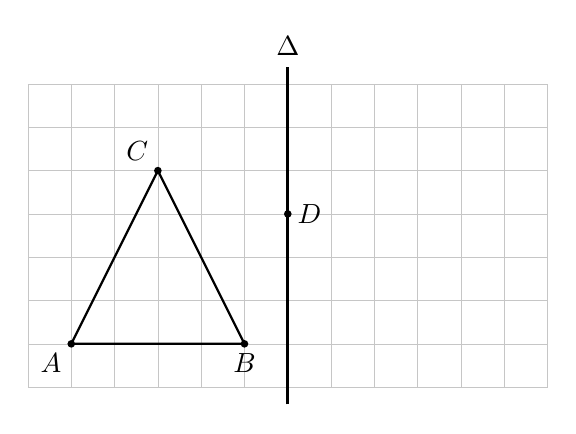
\begin{tikzpicture}[scale=0.55]
  \draw[gray!45,very thin] (0,0) grid (12,7);
  \draw[very thick] (6,-0.4)--(6,7.4) node[above] {$\Delta$};
  \draw[thick] (1,1)--(5,1)--(3,5)--cycle;
  \fill (1,1) circle (2.5pt) node[below left] {$A$};
  \fill (5,1) circle (2.5pt) node[below] {$B$};
  \fill (3,5) circle (2.5pt) node[above left] {$C$};
  \fill (6,4) circle (2.5pt) node[right] {$D$};
\end{tikzpicture}
\end{center}
\begin{enumerate}
  \item ابنِ النقاط $A'$ و $B'$ و $C'$ مناظرات $A$ و $B$ و $C$ بالنسبة إلى $\Delta$ ، ثم المثلث $A'B'C'$.
  \item احسب $AB$ ثم $A'B'$ بعدّ المربعات. ماذا تلاحظ ؟
  \item ما هي مناظرة النقطة $D$ بالنسبة إلى $\Delta$ ؟ علّل.
\end{enumerate}
\axsol
\begin{enumerate}[itemsep=14pt]
  \item\leavevmode
  \begin{prop}[البناء على الشبكة]
  $\Delta$ عمودي (رأسي)، فننتقل أفقيا : إذا كانت النقطة تبعد \ib{$n$ مربعات يسار $\Delta$} فمناظرتها تبعد \ib{$n$ مربعات يمين $\Delta$} على نفس السطر.
  \end{prop}
  \begin{itemize}
    \item $A$ تبعد $5$ مربعات عن $\Delta$ : نعدّ $5$ مربعات يمين $\Delta$ فنجد $A'$.
    \item $B$ تبعد مربعا واحدا عن $\Delta$ : $B'$ تبعد مربعا واحدا يمين $\Delta$.
    \item $C$ تبعد $3$ مربعات عن $\Delta$ : $C'$ تبعد $3$ مربعات يمين $\Delta$.
  \end{itemize}
  \begin{center}
  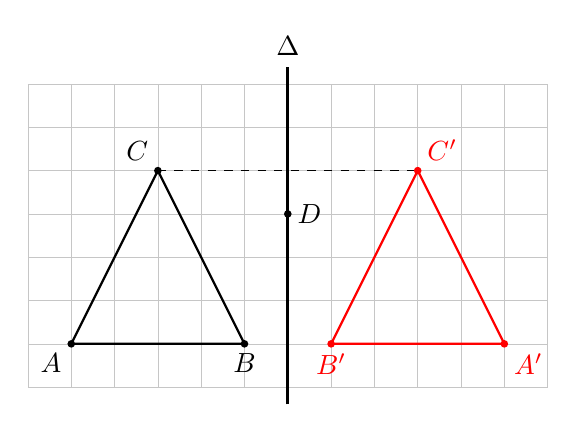
\begin{tikzpicture}[scale=0.55]
    \draw[gray!45,very thin] (0,0) grid (12,7);
    \draw[very thick] (6,-0.4)--(6,7.4) node[above] {$\Delta$};
    \draw[thick] (1,1)--(5,1)--(3,5)--cycle;
    \draw[thick,red] (11,1)--(7,1)--(9,5)--cycle;
    \draw[dashed] (3,5)--(9,5);
    \fill (1,1) circle (2.5pt) node[below left] {$A$};
    \fill (5,1) circle (2.5pt) node[below] {$B$};
    \fill (3,5) circle (2.5pt) node[above left] {$C$};
    \fill (6,4) circle (2.5pt) node[right] {$D$};
    \fill[red] (11,1) circle (2.5pt) node[below right] {$A'$};
    \fill[red] (7,1) circle (2.5pt) node[below] {$B'$};
    \fill[red] (9,5) circle (2.5pt) node[above right] {$C'$};
  \end{tikzpicture}
  \end{center}
  \item $AB=4$ وحدات (4 مربعات على السطر).

  $A'B'=4$ وحدات أيضا.

  نلاحظ أن \ib{$A'B'=AB$} : التناظر المحوري يحافظ على الأطوال.
  \item $D$ تنتمي إلى $\Delta$ ، وكل نقطة من المحور هي مناظرة نفسها : \ib{مناظرة $D$ هي $D$}.
\end{enumerate}
\end{corr}

\end{document}
